\documentclass[12pt]{scrreprt}

\usepackage{sty/preamble}
\usepackage{graphicx}
\usepackage{float}

\title{Manuale Utente}
\subtitle{CLIMATE MONITORING}
\author{
	\\Iuri Antico \textsl{matricola}:
	\texttt{753144}
	\and \\
	Beatrice Balzarini \textsl{matricola}:
	\texttt{752257}
	\and \\
	Michael Bernasconi \textsl{matricola}:
	\texttt{752259}
	\and \\
	Gabriele Borgia \textsl{matricola}:
	\texttt{753262}\\\\
}
\date{\today}

\begin{document}

	\maketitle

	\tableofcontents
	\listoffigures

	\chapter{Il Programma}
	\section{Introduzione}
		\textsl{Climate Monitoring} \`e un'applicazione finalizzata al monitoraggio di parametri climatici fornita da centri di monitoraggio sul territorio italiano, in grado di rendere disponibili, a operatori ambientali e comuni cittadini, i dati relativi alla propria zona di interesse.

		\subsection{Funzionamento generale dell'applicazione}
		L'applicazione offre diverse funzionalit\`a tra cui:
		\begin{itemize}
			\item la creazione di nuovi centri di monitoraggio climatico;
			\item l'inserimento di nuove misurazioni con i relativi parametri climatici;
			\item la visualizzazione delle aree geografiche presenti nel database;
			\item la visualizzazione di centri di monitoraggio presenti nel database;
			\item la visualizzazione delle misurazioni presenti nel database;
			\item la visualizzazione degli operatori registrati nel database;
		\end{itemize}
		\pagebreak
		I parametri climatici che possono essere rilevati e inseriti sono:
		\begin{itemize}
		\item \textsl{Vento}, la cui velocit\`a \`e espressa in km/h;
		\item \textsl{Umidit\`a}, misurata in percentuale (\%);
		\item \textsl{Pressione}, misurata in hPa;
		\item \textsl{Temperatura}, misurata in C°;
		\item \textsl{Precipitazione}, misurata in mm di pioggia;
		\item \textsl{Altitudine dei ghiacciai}, misurata in m;
		\item \textsl{Massa dei ghiacciai}, misurata in kg.
		\end{itemize}
		L'intensit\`a di ogni fenomeno climatico viene misurata su una scala che va da \textbf{1} (\textsl{critico}) a \textbf{5} (\textsl{ottimale}).
		
		Possono inoltre essere presenti delle note testuali (di massimo 256 caratteri) per descrivere con più precisione i dati geografici.
		
		L'applicazione permette:
		\begin{itemize}
		\item ai \textbf{\textsl{comuni cittadini}}, di visualizzare i parametri climatici di proprio interesse relativi a ciascuna area geografica;
		\item a \textbf{\textsl{operatori autorizzati}}, di gestire le aree di interesse inserendo i vari parametri climatici.
		\end{itemize}
		Inoltre questi ultimi hanno la possibilit\`a di registrarsi, creare nuovi centri di monitoraggio ed aggiungervi aree di interesse.

	\pagebreak

	\section{Requisiti minimi\index{Requisiti minimi}}
		Per eseguire l’applicazione \`e necessario avere a disposizione:
		\begin{itemize}
			\item Java JDK 17 o superiore;
			\item un sistema operativo a 64 bit;
			\item un terminale.
		\end{itemize}

	
	\section{Troubleshooting}
		\subsection{Problemi durante l'avvio}
		Se l'applicazione non si dovesse avviare correttamente:
		\begin{itemize}
			\item assicurarsi di star utilizzando \textsl{Java JDK 17} o superiore;
			\item assicurarsi che le variabili d'ambiente siano state impostate correttamente;
			\item assicurarsi di aver seguito in maniera corretta le istruzioni indicate nel paragrafo precedente:
			\begin{itemize}
				\item tenere presente che non \`e possibile aprire l'applicazione tramite doppio click;
				\item assicurarsi che il comando di avvio coincida con quello mostrato e che venga eseguito nell'indirizzo corretto.
			\end{itemize}
		\end{itemize}
		
		Nel caso l'applicazione non dovesse avviarsi per qualsiasi altro motivo sono disponibili i file sorgente che possono essere visualizzati modificati tramite qualsiasi IDE.
		
		\subsection{Inserimento di nomi propri nei comandi}
		Quando si inseriscono nei comandi nomi propri (ad esempio di citt\`a) \`e necessario prestare attenzione alla lettera maiuscola iniziale, in quanto alcune funzioni sono \textsl{case sensitive} e potrebbero non funzionare correttamente.
	
	\section{Avviare l'applicazione}
	
	Per avviare l'applicazione \`e necessario:
	\begin{enumerate}
		\item cliccare con il tasto destro la cartella \textsl{UniLab} e selezionare "\textsl{Apri nel Terminale}" (o "\textsl{Open in Terminal}"):
		\begin{figure}[H]
			\centering
			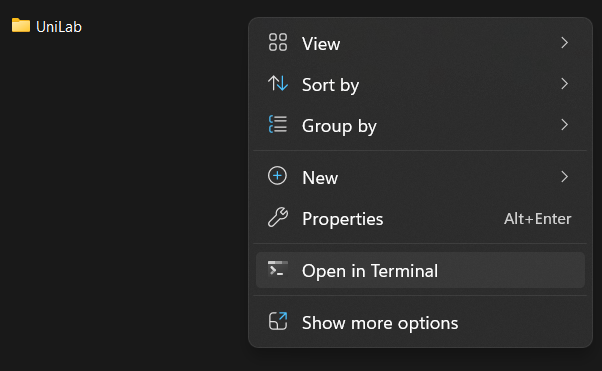
\includegraphics[width=0.7\linewidth]{Screen/aprinelterminale}
			\caption{Aprire la cartella nel terminale}
			\label{fig:aprinelterminale}
		\end{figure}
		\item una volta aperto il terminale digitare il comando
		\verb! .\UniLab.exe.! e premere invio.
		\begin{figure}[H]
			\centering
			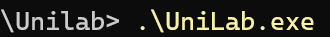
\includegraphics[width=0.3\linewidth]{Screen/avviocom}
			\caption{Comando di avvio dell'applicazione}
			\label{fig:avviocom}
		\end{figure}
	\end{enumerate}
	
	\section{Schermata principale}

	
	All'avvio dell'applicazione compare la seguente schermata, dove \`e possibile visualizzare il menu principale del programma.
	\begin{figure}[H]
		\centering
		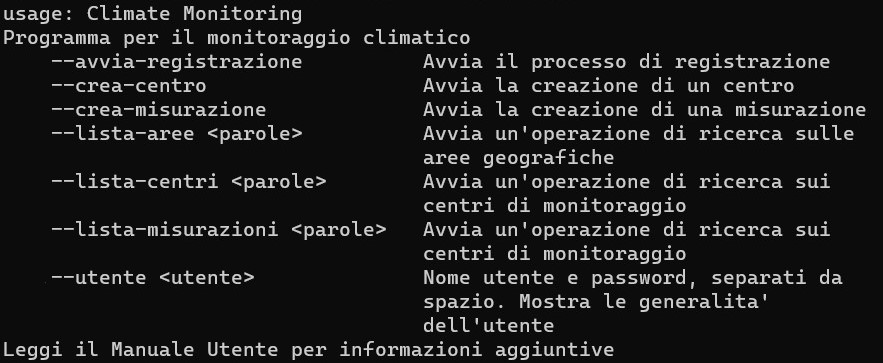
\includegraphics[width=0.9\linewidth]{Screen/schermataprincipale}
		\caption{Schermata principale}
		\label{fig:schermataprincipale}
	\end{figure}	
		
	\section{Menù principale}
	
		\subsection{-$ $-avvia-registrazione}
	
		Per avviare questo comando \`e necessario digitare nel terminale\\
		\verb!    .\UniLab.exe --avvia-registrazione!\\
		\begin{figure}[H]
			\centering
			
\includegraphics[width=0.5\linewidth]{Screen/registrazione}
			\caption{Registrazione}
			\label{fig:registrazione (non implementata)}
		\end{figure}
			Questa funzione non \`e stata implementata, per ulteriori informazioni consultare il \textsl{Manuale Tecnico}. 
		
		\subsection{-$ $-crea-centro}
		Questa funzione permette di creare un centro di monitoraggio e salvarlo nel database.
		
		Se \`e la prima volta che viene inserito un centro di monitoraggio nel database \`e necessario seguire le istruzioni seguenti:
		\begin{enumerate}
			
		\item verificare che non esista un file chiamato "\textsl{centro.ini}" nella cartella \textsl{UniLab}: qualora esista \`e necessario seguire le istruzioni illustrate nel prossimo paragrafo, in quanto \`e gi\`a stato inserito almeno un centro di monitoraggio nel database;
		\item avviare il comando digitando sul terminale
		\\\verb!    .\UniLab.exe --crea-centro!\\ e premere il tasto invio.
		\begin{figure}[H]
			\centering
			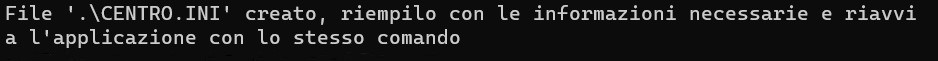
\includegraphics[width=1\linewidth]{Screen/creacentrocom}
			\caption{Risultato del comando -$ $-crea-centro}
			\label{fig:creacentrocom}
		\end{figure}
		\item aprire (tramite un visualizzatore di file di testo) il file \textsl{centro.ini}.

		\item inserire nel file i seguenti dati:
		\begin{figure}[H]
			\centering
			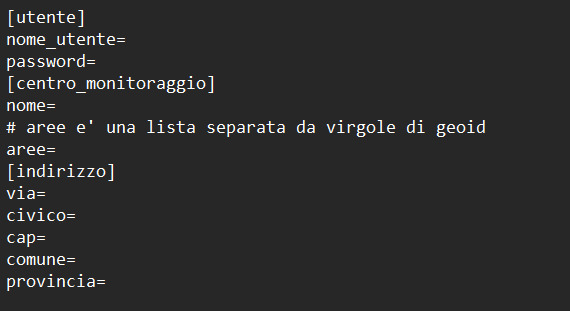
\includegraphics[width=0.7\linewidth]{Screen/creacentroini}
			\caption{Creazione del file .ini relativo ai centri di monitoraggio}
			\label{fig:creacentroini}
		\end{figure}
			Nelle voci \verb!nome_utente! e \verb!password! \`e necessario inserire rispettivamente \verb!Civile! e \verb!civile00!, in modo da essere riconosciuti dal sistema come operatore e avere la possibilit\`a di creare un nuovo centro di monitoraggio.
			\item salvare e chiudere il file \textsl{centro.ini};
			\item tornare sulla schermata del terminale e rieseguire il comando
			\\\verb!    .\UniLab.exe --crea-centro!\\
		\end{enumerate}
		
		Se un centro di monitoraggio \`e gi\`a stato precedentemente creato e si vuole aggiungerne un altro, \`e necessario:
		\begin{enumerate}
			\item aprire il file \textsl{centro.ini};
			\item modificare i dati relativi al nuovo centro di monitoraggio (nome utente e password devono sempre essere \verb!Civile! e \verb!civile00!);
			\item salvare e chiudere il file;
			\item rieseguire il comando \\\verb!    .\UniLab.exe --crea-centro!
		\end{enumerate}
		A questo punto, se tutte le istruzioni sono state eseguite correttamente, i dati relativi al nuovo centro di monitoraggio saranno stati acquisiti correttamente dall'applicazione.
		\pagebreak
		\subsection{-$ $-crea-misurazione}
		
		Questa funzione permette di creare una misurazione e salvarla nel database.
		
		Se \`e la prima volta che viene inserita una misurazione nel database \`e necessario seguire le istruzioni seguenti:
		\begin{enumerate}
			\item verificare che non esista un file chiamato "\textsl{misurazione.ini}" nella cartella \textsl{UniLab}: qualora esista \`e necessario seguire le istruzioni illustrate nel prossimo paragrafo, in quanto \`e gi\`a stata inserita almeno una misurazione nel database;
			\item avviare il comando digitando sul terminale
			\\\verb!    .\UniLab.exe --crea-misurazione!\\ e premere il tasto invio.
			\begin{figure}[H]
				\centering
				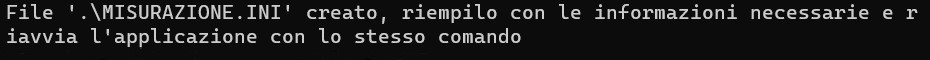
\includegraphics[width=1\linewidth]{Screen/creamisurazionecom}
				\caption{Risultato del comando -$ $-crea-misurazione}
				\label{fig:creamisurazionecom}
			\end{figure}
			
			\item aprire (tramite un visualizzatore di file di testo) il file \textsl{misurazione.ini}.
			\pagebreak
			\item inserire nel file i seguenti dati:
			\begin{figure}[H]
				\centering
				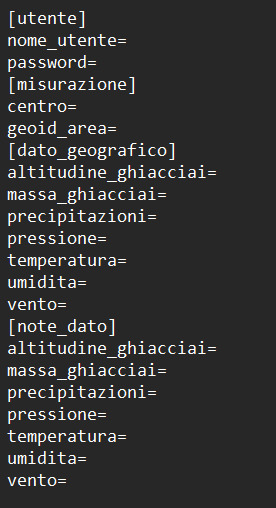
\includegraphics[width=0.4\linewidth]{Screen/creamisurazioneini}
				\caption{Creazione del file .ini relativo alle misurazioni}
				\label{fig:creamisurazioneini}
			\end{figure}
			Nelle voci \verb!nome_utente! e \verb!password! \`e necessario inserire rispettivamente \verb!Civile! e \verb!civile00!, in modo da essere riconosciuti dal sistema come operatore e avere la possibilit\`a di creare una nuova misurazione.
			\item salvare e chiudere il file \textsl{misurazione.ini};
			\item tornare sulla schermata del terminale e rieseguire il comando
			\\\verb!    .\UniLab.exe --crea-misurazione!
		\end{enumerate}
		\pagebreak
		Se una misurazione \`e gi\`a stata precedentemente creata e si vuole aggiungerne un'altra, \`e necessario:
		\begin{enumerate}
			\item aprire il file \textsl{misurazione.ini};
			\item modificare i dati relativi alla nuova misurazione (nome utente e password devono sempre essere \verb!Civile! e \verb!civile00!);
			\item salvare e chiudere il file;
			\item rieseguire il comando \\\verb!    .\UniLab.exe --crea-misurazione!
		\end{enumerate}
		A questo punto, se tutte le istruzioni sono state eseguite correttamente, i dati relativi alla nuova misurazione saranno stati acquisiti correttamente dall'applicazione.
		\pagebreak
		\subsection{-$ $-lista-aree <parole>}
		
		Questa funzione permette di visualizzare le aree geografiche presenti nel database il cui nome contiene la/e parola/e fornita/e nel comando.
		
		Se si vogliono visualizzare tutte le aree geografiche presenti nel database \`e necessario eseguire il comando \\\verb!    .\UniLab.exe --lista-aree!
		
		\begin{figure}[H]
			\centering
			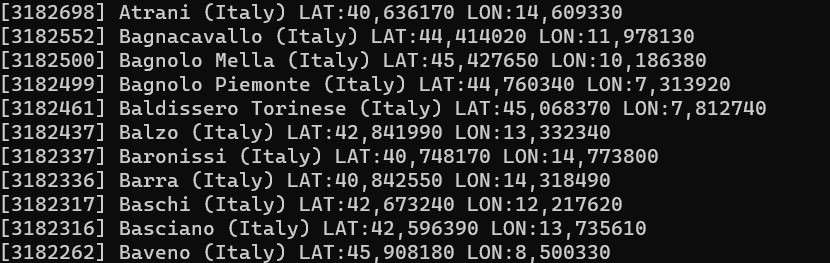
\includegraphics[width=0.8\linewidth]{Screen/listaaree}
			\caption{Alcune delle aree geografiche presenti nel database}
			\label{fig:listaaree}
		\end{figure}
		Se si vuole visualizzare delle determinate aree geografiche \`e necessario eseguire il comando \\\verb!    .\UniLab.exe --lista-aree <parole>!\\
		Al posto di \verb!<parole>! \`e necessario inserire il nome delle aree geografiche di interesse.
			
		Di seguito viene mostrato un esempio nel quale vengono visualizzate tutte le aree geografiche il cui nome contiene "\textsl{mil}", nonché il risultato del comando \\\verb!.\UniLab.exe --lista-aree mil!
		\begin{figure}[H]
			\centering
			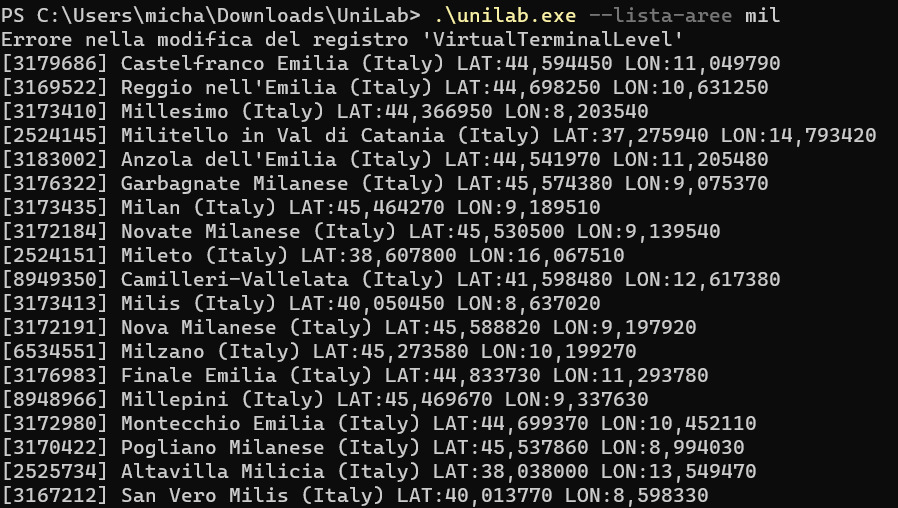
\includegraphics[width=0.8\linewidth]{Screen/listaareemil}
			\caption{Risultato della ricerca di aree geografiche con "mil"}
			\label{fig:listaareemil}
		\end{figure}
		 
		\pagebreak
		\subsection{-$ $-lista-centri <parole>}
		Questa funzione permette di visualizzare i centri di monitoraggio presenti nel database il cui nome contiene la/e parola/e fornita/e nel comando.
		
		Se si vogliono visualizzare tutti i centri di monitoraggio presenti nel database \`e necessario eseguire il comando \\\verb!    .\UniLab.exe --lista-centri!
		
		\begin{figure}[H]
			\centering
			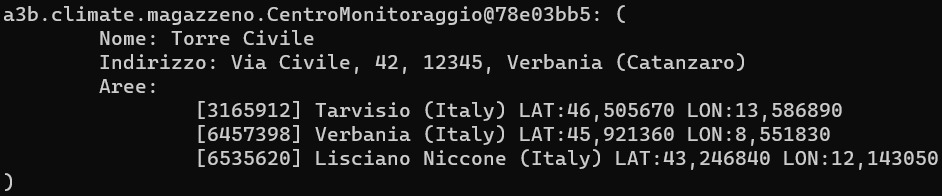
\includegraphics[width=0.9\linewidth]{Screen/listacentri}
			\caption{Alcuni dei centri di monitoraggio presenti nel database}
			\label{fig:listacentri}
		\end{figure}
		
		Se si vuole visualizzare dei determinati centri di monitoraggio \`e necessario eseguire il comando \\\verb!    .\UniLab.exe --lista-centri <parole>!
		
		Al posto di \verb!<parole>! \`e necessario inserire il nome dei centri di monitoraggio di interesse.
		
		Questo comando funziona in maniera analoga al precedente, per tanto se si necessita un esempio del funzionamento si consiglia di consultare la documentazione della funzione \verb!.\UniLab.exe --lista-aree <parole>!.
		\pagebreak
		\subsection{-$ $-lista-misurazioni <parole>}
		Questa funzione permette di visualizzare le misurazioni presenti nel database che contengono la/e parola/e fornita/e nel comando.
		
		Se si vogliono visualizzare tutte le misurazioni presenti nel database \`e necessario eseguire il comando \\\verb!    .\UniLab.exe --lista-misurazioni!
		
		\begin{figure}[H]
			\centering
			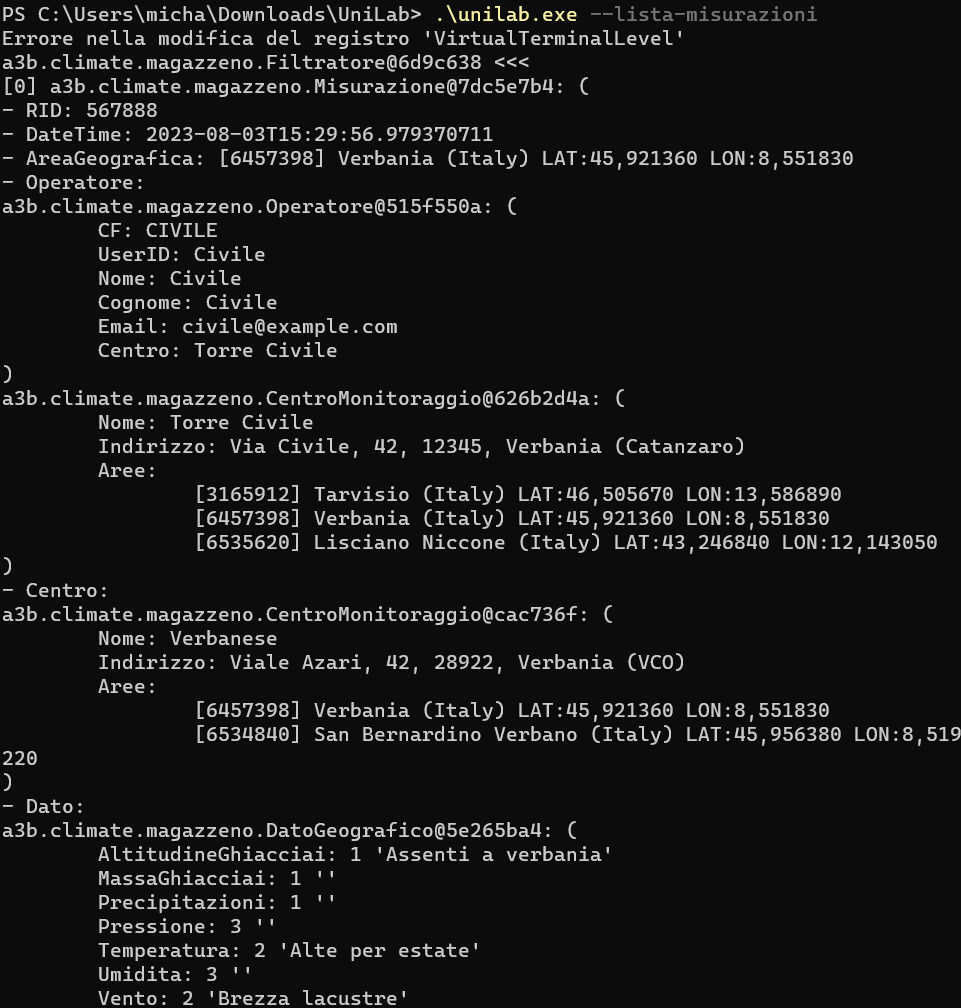
\includegraphics[width=0.9\linewidth]{Screen/listamisurazioni}
			\caption{Alcune delle misurazioni nel database}
			\label{fig:listamisurazioni}
		\end{figure}
		\pagebreak
		Se si vuole visualizzare delle determinate misurazioni \`e necessario eseguire il comando \\\verb!    .\UniLab.exe --lista-misurazioni <parole>!
		
		Al posto di \verb!<parole>! \`e necessario inserire le misurazioni di interesse.
		
		Questo comando funziona in maniera analoga al precedente, per tanto se si necessita un esempio del funzionamento si consiglia di consultare la documentazione della funzione \verb!.\UniLab.exe --lista-aree <parole>!.
		\pagebreak
		\subsection{-$ $-utente <utente>}
		Questo comando permette di visualizzare il profilo dell'operatore.
		
		Per avviare questa funzione \`e necessario digitare il seguente comando
		\\\verb!    .\UniLab.exe --utente!\\
		Accanto a \verb!--utente! \`e necessario inserire nome utente e password (che devono essere \verb!Civile! e \verb!civile00!) separati da uno spazio, come riportato nel seguente esempio:
		\begin{figure}[H]
			\centering
			
\includegraphics[width=0.6\linewidth]{Screen/utentecom}
			\caption{Comando -$ $-utente}
			\label{fig:utentecom}
		\end{figure}
		
		Di seguito viene mostrato il risultato del comando.
		
		\begin{figure}[H]
			\centering
			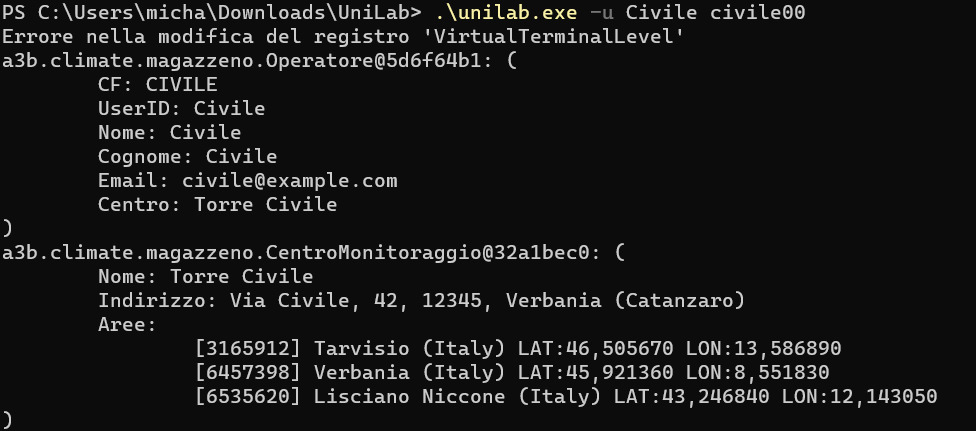
\includegraphics[width=0.9\linewidth]{Screen/utente}
			\caption{Risultato dei comandi -u e -$ $-utente}
			\label{fig:utente}
		\end{figure}
		
	\pagebreak
	\subsection{Esci}
	Per uscire dall’applicazione \`e sufficiente chiudere il terminale, cliccando sull’icona a croce ("\textsl{Chiudi}" o "\textsl{Close}") in alto a destra:
	\begin{figure}[H]
		\centering
		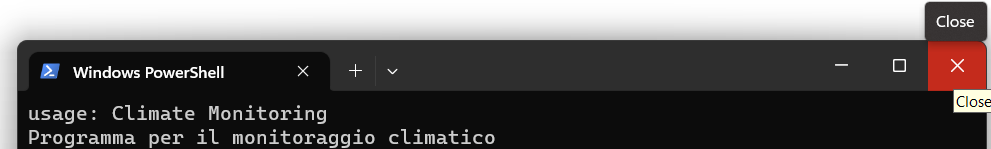
\includegraphics[width=0.9\linewidth]{Screen/esci}
		\caption{Icona per chiudere il terminale (uscire dal programma)}
		\label{fig:esci}
	\end{figure}

	\chapter{Limiti della soluzione sviluppata}
	Nello sviluppo dell'applicazione sono state riscontrate delle difficolt\`a nella implementazione di alcune funzioni:
	\begin{itemize}
		\item \textbf{Registrazione non implementata}:\\Il programma fornisce dei parametri di default per la registrazione in quanto non \`e stato possibile implementare una funzione per registrare un nuovo operatore con credenziali a scelta dall'utente.\\Ulteriori informazioni nel \textsl{Manuale Tecnico}.
		
		\item \textbf{Verifica della correttezza degli indirizzi assente}:\\Non potendo accedere direttamente al database contenente le aree geografiche, non \`e possibile verificare che la provincia relativa ai centri di monitoraggio sia corretta dal punto di vista geografico.
	\end{itemize}

	
	

	\nocite{IuriTex}
	\bibliographystyle{alpha}
	\bibliography{bib/biblio}
	\printindex

\end{document}



